\documentclass[draft]{article}
%\usepackage[final]{graphics}
% final means "include the picture".  draft means "put a space with filename"
\usepackage[final]{graphicx}
\usepackage{latexsym}
\usepackage{amssymb}
\usepackage{amsmath}
%\usepackage{showkeys}  %shows labels in margins see Gratzer p. 249
\setlength{\abovecaptionskip}{0pt}
\setlength{\parindent}{0cm} % no indent for paragraphs
\setlength{\parskip}{1.5ex} % more space between paragraphs.
\setlength{\textwidth}{7in} % width of text 
\setlength{\oddsidemargin}{0pt}  % makes margin narrower
\title{Double Pendulum as Rigid Bodies}
\author{Erik Neumann\\
erikn@myphysicslab.com}
\date{April 2, 2011}
\begin{document}

\maketitle
%===============================================================
\section{Introduction}

This is a derivation of the equations of motion for a double pendulum where we regard the pendulums as rigid bodies.  In an alternate double pendulum model, the so-called ``ideal double pendulum'', the two pendulums are modelled as massless rods with a point mass at the end of each pendulum rod.  The present rigid body model of the double pendulum allows for more realistic configurations, because the pendulums can have any distribution of mass and can be connected together at any point.  The mass distribution is reflected in the rotational inertia of each pendulum.  By contrast in the ideal double pendulum model, the rotational inertia is zero for each pendulum and the connection must be at the end points of the massless rods.

\begin{figure}
    \centering
    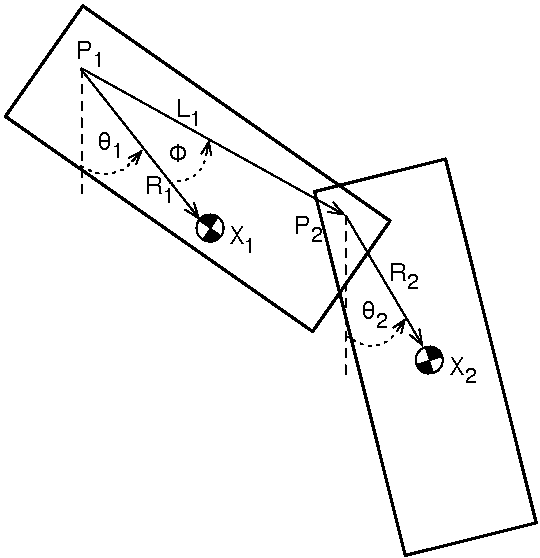
\includegraphics[width=0.40 \textwidth]{Rigid_Double_Pendulum_fig_1.pdf}
    \caption{Rigid Body Double Pendulum Model} \label{fig_1}
\end{figure}

Please refer to figure \ref{fig_1} below.

Let $\mathbf{i}$ be the unit vector along the $x$ axis, and let $\mathbf{j}$ be the unit vector along the $y$ axis.  We regard $y$ as increasing upwards (this is the usual mathematical convention, as opposed to computer graphics systems which often have $y$ increasing downwards).  

The fixed pivot, which we name pivot 1, is at location $\mathbf{P_1}$.  Pivot 2 is the moving pivot point connecting the two pendulums at location $\mathbf{P_2}$.

Let pendulum 1 be the upper pendulum.  It is connected to a fixed location at pivot 1, and connected to the lower pendulum at pivot 2.\\
Let $\mathbf{X_1} = x_1 \mathbf{i} + y_1 \mathbf{j}$ be the location of the center of mass of pendulum 1.\\
Let $\mathbf{R_1}$ be the vector from pivot 1 to the center of mass of pendulum 1, with length $R_1$.\\
Let $\theta_1$ be the angle at pivot 1 between $\mathbf{R_1}$ and the downward vertical position.\\
Let $\mathbf{L_1}$ be the vector from pivot 1 to pivot 2, with length $L_1$.\\
Let $\phi$ be the angle from vector $\mathbf{R_1}$ to $\mathbf{L_1}$.  Note that $\phi$ is a constant.

Let pendulum 2 be the lower pendulum.  It is connected to the upper pendulum at pivot 2.\\
Let $\mathbf{X_2} = x_2 \mathbf{i} + y_2 \mathbf{j}$ be the location of the center of mass of pendulum 2.\\
Let $\mathbf{R_2}$ be the vector from pivot 2 to the center of mass of pendulum 2, with length $R_2$.\\
Let $\theta_2$ be the angle at pivot 2 between $\mathbf{R_2}$ and the downward vertical position.

Let $m_1$, $m_2$ be the mass of pendulum 1 and 2 respectively.\\
Let $I_1$, $I_2$ be the rotational inertia about the center of mass of pendulum 1 and 2 respectively.

%===============================================================
\section{Kinematics}
We have the following relationships just from the geometry of the double pendulum, without using any information about forces. 
\[
\mathbf{R_1} = R_1 \sin(\theta_1) \mathbf{i} - R_1 \cos(\theta_1) \mathbf{j}
\]
\[
\mathbf{R_2} = R_2 \sin(\theta_2) \mathbf{i} - R_2 \cos(\theta_2) \mathbf{j}
\]
\[
\mathbf{L_1} = L_1 \sin(\theta_1+\phi) \mathbf{i} - L_1 \cos(\theta_1+\phi) \mathbf{j}
\]

\[
\mathbf{X_1} = \mathbf{R_1}
\]
\[
x_1 = R_1 \sin(\theta_1)
\]
\[
y_1 = -R_1 \cos(\theta_1)
\]
\[
\mathbf{X_2} = \mathbf{L_1} + \mathbf{R_2}
\]
\[
x_2 = L_1 \sin(\theta_1+\phi) + R_2 \sin(\theta_2)  
\]
\[
y_2 = -L_1 \cos(\theta_1+\phi) - R_2 \cos(\theta_2) 
\]

Take the first derivative with respect to time to get velocity.

\[
\mathbf{X_1'} = \mathbf{R_1'}
\]
\[
x_1' = \theta_1' R_1 \cos(\theta_1)
\]
\[
y_1' = \theta_1' R_1 \sin(\theta_1)
\]
\[
\mathbf{X_2'} = \mathbf{L_1'} + \mathbf{R_2'}
\]
\[
x_2' = \theta_1' L_1 \cos(\theta_1+\phi) + \theta_2' R_2 \cos(\theta_2)
\]
\[
y_2' = \theta_1' L_1 \sin(\theta_1+\phi) + \theta_2' R_2 \sin(\theta_2)
\]

Take the second derivative with respect to time to get acceleration.

\[
\mathbf{X_1''} = \mathbf{R_1''}
\]
\begin{equation}\label{E01}
x_1'' = -\theta_1'^2 R_1 \sin(\theta_1) + \theta_1'' R_1 \cos(\theta_1)
\end{equation}
\begin{equation}\label{E02}
y_1'' = \theta_1'^2 R_1 \cos(\theta_1) + \theta_1'' R_1 \sin(\theta_1)
\end{equation}
\[
\mathbf{X_2''} = \mathbf{L_1''} + \mathbf{R_2''}
\]
\begin{equation}\label{E1}
x_2'' = -\theta_1'^2 L_1 \sin(\theta_1+\phi) + \theta_1'' L_1 \cos(\theta_1+\phi)
- \theta_2'^2 R_2 \sin(\theta_2) + \theta_2'' R_2 \cos(\theta_2)
\end{equation}
\begin{equation}\label{E2}
y_2'' = \theta_1'^2 L_1 \cos(\theta_1+\phi) + \theta_1'' L_1 \sin(\theta_1+\phi)
+ \theta_2'^2 R_2 \cos(\theta_2) + \theta_2'' R_2 \sin(\theta_2)
\end{equation}


%===============================================================
\section{Forces}

Let $\mathbf{T_1} = T_{1x} \mathbf{i} + T_{1y} \mathbf{j}$ be the force vector operating on pendulum 1 at pivot 1.\\
Let $\mathbf{T_2} = T_{2x} \mathbf{i} + T_{2y} \mathbf{j}$ be the force vector operating on pendulum 1 at pivot 2.
Then by Newton's law of equal and opposite reaction, $-\mathbf{T_2}$ is the force vector operating on pendulum 2 at pivot 2.

From Newton's laws of motion we can write the following force equations:
\[
m_1 \mathbf{X_1}'' = \mathbf{T_1} + \mathbf{T_2} - m_1 g \mathbf{j}
\]
\begin{equation}\label{E3}
m_1 x_1'' = T_{1x} + T_{2x}
\end{equation}
\begin{equation}\label{E4}
m_1 y_1'' = T_{1y} + T_{2y} - m_1 g
\end{equation}
\begin{multline}\label{E5}
  I_1 \theta_1'' = (-\mathbf{R_1}) \times \mathbf{T_1} + (\mathbf{L_1 - R_1}) \times \mathbf{T_2} \\
  = -(R_1 \sin(\theta_1) T_{1y} + R_1 \cos(\theta_1) T_{1x}) \\
  + (L_1 \sin(\theta_1+\phi)- R_1 \sin(\theta_1))  T_{2y} 
  + (L_1 \cos(\theta_1+\phi) - R_1 \cos(\theta_1)) T_{2x}
\end{multline}
\[
m_2 \mathbf{X_2}'' = -\mathbf{T_2} - m_2 g \mathbf{j}
\]
\begin{equation}\label{E6}
m_2 x_2'' = -T_{2x}
\end{equation}
\begin{equation}\label{E7}
m_2 y_2'' = -T_{2y} - m_2 g
\end{equation}
\begin{equation}\label{E8}
  I_2 \theta_2'' = (-\mathbf{R_2}) \times (-\mathbf{T_2}) 
  = R_2 \sin(\theta_2) T_{2y} + R_2 \cos(\theta_2) T_{2x}
\end{equation}

To derive these force equations we used Newton's law of motion $\mathbf{F} = m \mathbf{a}$ and the rotational version for angular torque $I \theta'' = \tau$.  For more about how to calculate the torque see \texttt{http://www.myphysicslab.com/collision.html}.

%===============================================================
\section{Equations of Motion}

Substitute the four equations (\ref{E01}) thru (\ref{E2}) into the six equations (\ref{E3}) thru (\ref{E8}) to eliminate the unknowns $x_1''$, $y_1''$, $x_2''$, $y_2''$.  This gives us modified versions of the six equations (\ref{E3}) thru (\ref{E8}) with  six unknowns: $T_{1x}$, $T_{2x}$,  $T_{1y}$, $T_{2y}$, $\theta_1''$,  $\theta_2''$.  We then solve for $\theta_1''$, $\theta_2''$ and eliminate the other four unknowns.  See the accompanying Mathematica notebook \texttt{Rigid\_Double\_Pendulum\_Algebra.nb} for the calculations.

\small
\begin{multline}
\theta_1'' = -\Big(2 g m_1 R_1 (I_2 + m_2 R_2^2) \sin(\theta_1) + L_1 m_2 \Big(g (2 I_2 + m_2 R_2^2) \sin(\theta_1 + \phi) + \\
R_2 \Big(g m_2 R_2 \sin(\theta_1 - 2 \theta_2 + \phi) + 2 (\theta_2'^2 (I_2 + m_2 R_2^2) +
\theta_1'^2 L_1 m_2 R_2 \cos(\theta_1 - \theta_2 + \phi)) \sin(\theta_1 - \theta_2 + \phi)
\Big)\Big)\Big)\\
\Big/
\Big(2 I_2 L_1^2 m_2 + 2 I_2 m_1 R_1^2 + 
L_1^2 m_2^2 R_2^2 + 2 m_1 m_2 R_1^2 R_2^2 + 2 I_1 (I_2 + m_2 R_2^2) - 
L_1^2 m_2^2 R_2^2 \cos(2 (\theta_1 - \theta_2 + \phi))\Big) 
\end{multline}

\begin{multline}
\theta_2'' = \Big(m_2 R_2 \Big(-(g (2 I_1 + L_1^2 m_2 + 2 m_1 R_1^2) \sin(\theta_2)) + \\
L_1 \Big(g m_1 R_1 \sin(\theta_2 - \phi) + 2 \theta_1'^2 (I_1 + L_1^2 m_2 + m_1 R_1^2) \sin(\theta_1 - \theta_2 + \phi) + \\
\theta_2'^2 L_1 m_2 R_2 \sin(2 (\theta_1 - \theta_2 + \phi)) + g m_1 R_1 \sin(2 \theta_1 - \theta_2 + \phi) + 
g L_1 m_2 \sin(2 \theta_1 - \theta_2 + 2 \phi)\Big)\Big)\Big)\\
\Big/
\Big(2 I_2 L_1^2 m_2 + 2 I_2 m_1 R_1^2 + L_1^2 m_2^2 R_2^2 + 
2 m_1 m_2 R_1^2 R_2^2 + 2 I_1 (I_2 + m_2 R_2^2) - L_1^2 m_2^2 R_2^2 \cos(2 (\theta_1 - \theta_2 + \phi))\Big)
\end{multline}

Do these equations match the ideal double pendulum equations? Yes.

In the ideal double pendulum there are two point masses at the end of each pendulum.  This corresponds to setting $L_1=R_1$, $\phi=0$, and having rotational inertia be zero for both pendulums.  If we substitute these values into the above equations, we do indeed get the ideal double pendulum equations (see the Mathematica document).




\end{document}
